\subsection{Задание 2. Параметры согласованного фильтра и выходного сигнала}
В этом задании изучаются характеристики согласованных фильтров,
соответствующих каждому из сигналов, рассмотренных в задании №1. Кроме
того, исследуются вид и свойства выходных сигналов. Учитывая, что при
расширении фазового спектра длительность сигнала увеличивается, а при
уменьшении до нуля – укорачивается, в данном задании необходимо
внимательно проследить за укорочением сигнала. Самый короткий и самый
большой по амплитуде он должен получиться при нулевом фазовом спектре


Рекомендации по анализу результатов эксперимента
\begin{itemize}
    \item Как коэффициент передачи по амплитуде $\abs{K(\omega)}$ фильтра и фазовые
    сдвиги $\varphi(\omega)$, вносимые фильтром в соответствующую гармонику,
    связаны с амплитудным и фазовым спектром сигнала?
    \item Как связан выходной сигнал и его амплитудный и фазовый спектр с
    характеристиками выходного сигнала? Сравнить длительности
    входного и выходного сигналов.
    \item Какой вид имеет импульсная переходная характеристика
    согласованного фильтра?
    \item Какой фазовый спектр и база выходного сигнала? 
\end{itemize}



\subsubsection{Прямоугольный видеоимпульс}
\begin{figure}[H]
    \centering
    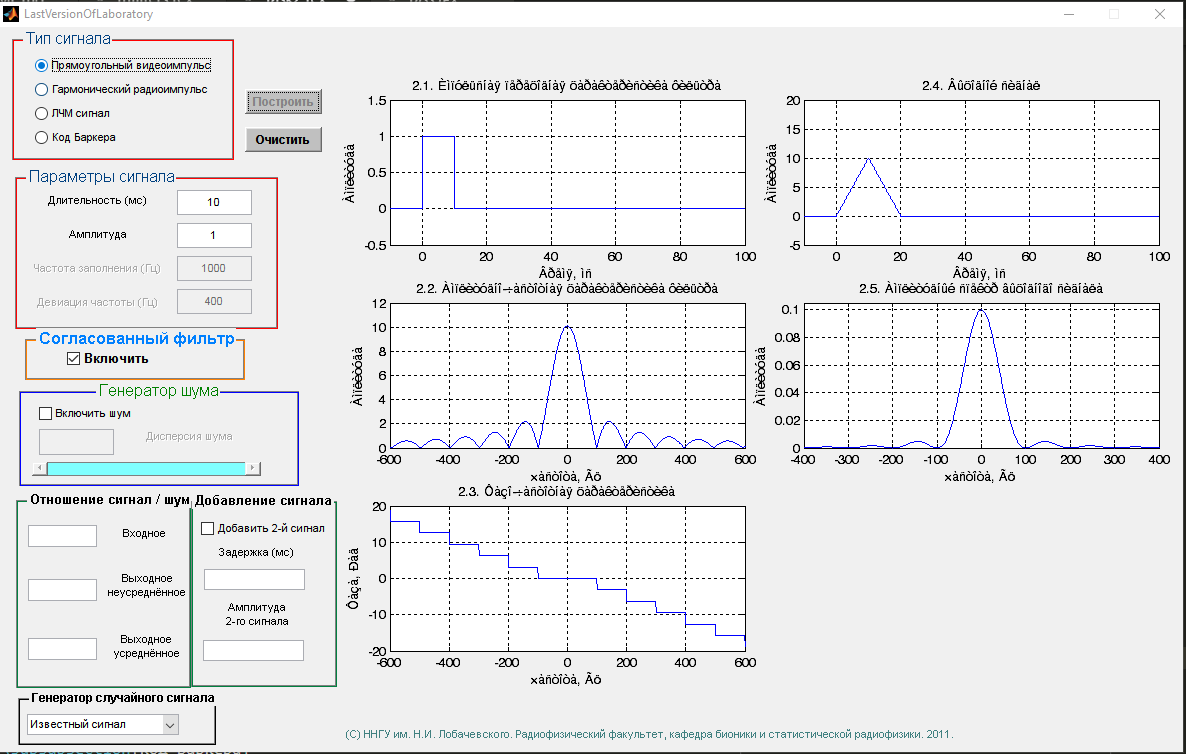
\includegraphics[width=0.9\linewidth]{imgs/task_2/t2s1_10.png}
    \caption{10 мс}
    \label{fig:task_2_1_10}
\end{figure}
\begin{figure}[H]
    \centering
    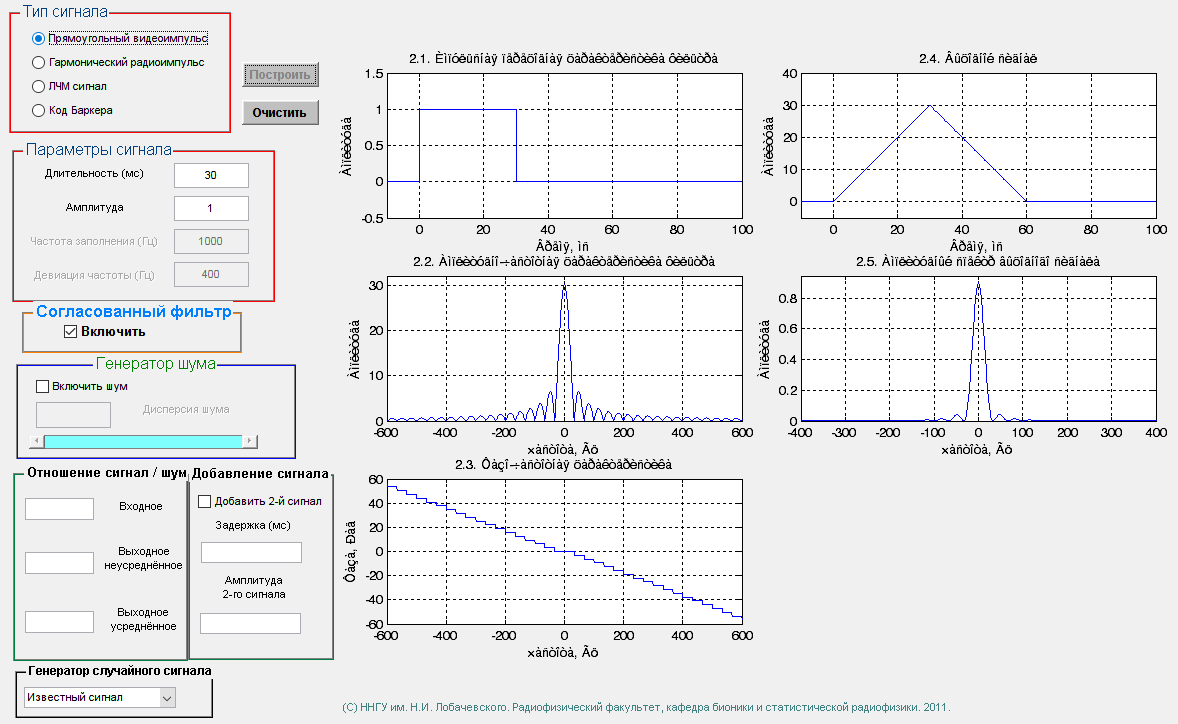
\includegraphics[width=0.9\linewidth]{imgs/task_2/t2s1_30.png}
    \caption{30 мс}
    \label{fig:task_2_1_30}
\end{figure}
АЧХ $\abs{K(i \omega)}$ и ФЧХ $\varphi (\omega)$ согласованного фильтра
\begin{equation}
    \abs{K(i \omega)} = \abs{C_0} \cdot \abs{C_m(i \omega)}, \quad
    \varphi (\omega) = -\varphi_m  -\omega t + arg(C_0),
\end{equation}
где $C_m, \varphi_m $ - амплитудный и фазовый спектры входного сигнала $m(t)$.
\begin{enumerate}
    \item 
    \item 
    \item 
    \item 
\end{enumerate}


\subsubsection{Прямоугольный видеоимпульс с гармоническим заполнением}
\begin{figure}[H]
    \centering
    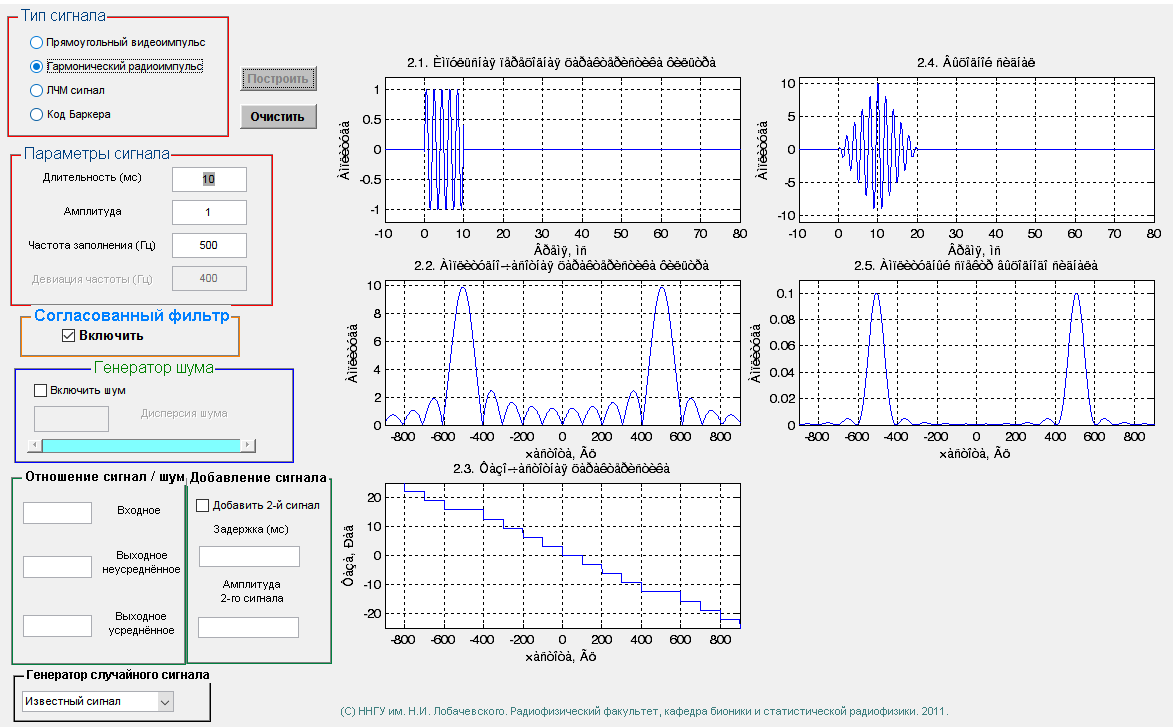
\includegraphics[width=0.9\linewidth]{imgs/task_2/t2s2_10.png}
    \caption{10 мс}
    \label{fig:task_2_2_10}
\end{figure}
\begin{figure}[H]
    \centering
    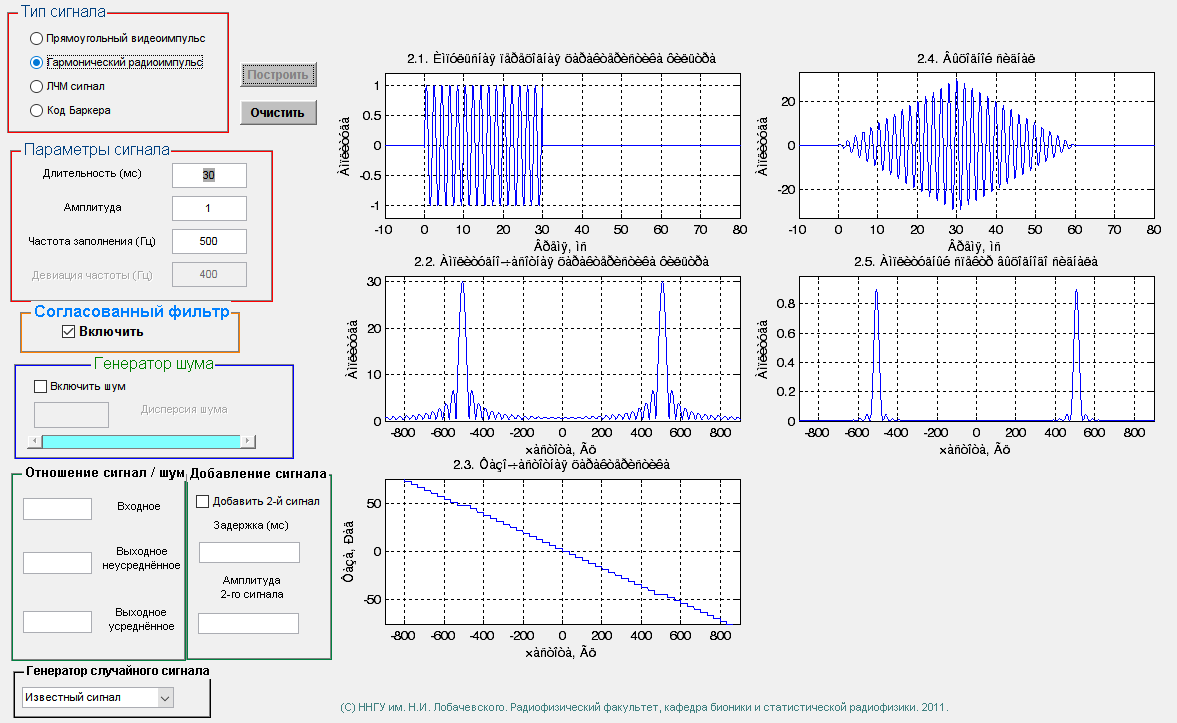
\includegraphics[width=0.9\linewidth]{imgs/task_2/t2s2_30.png}
    \caption{30 мс}
    \label{fig:task_2_2_30}
\end{figure}

\begin{enumerate}
    \item 
    \item 
    \item 
    \item 
\end{enumerate}


\subsubsection{ЛЧМ сигнал}
\begin{figure}[H]
    \centering
    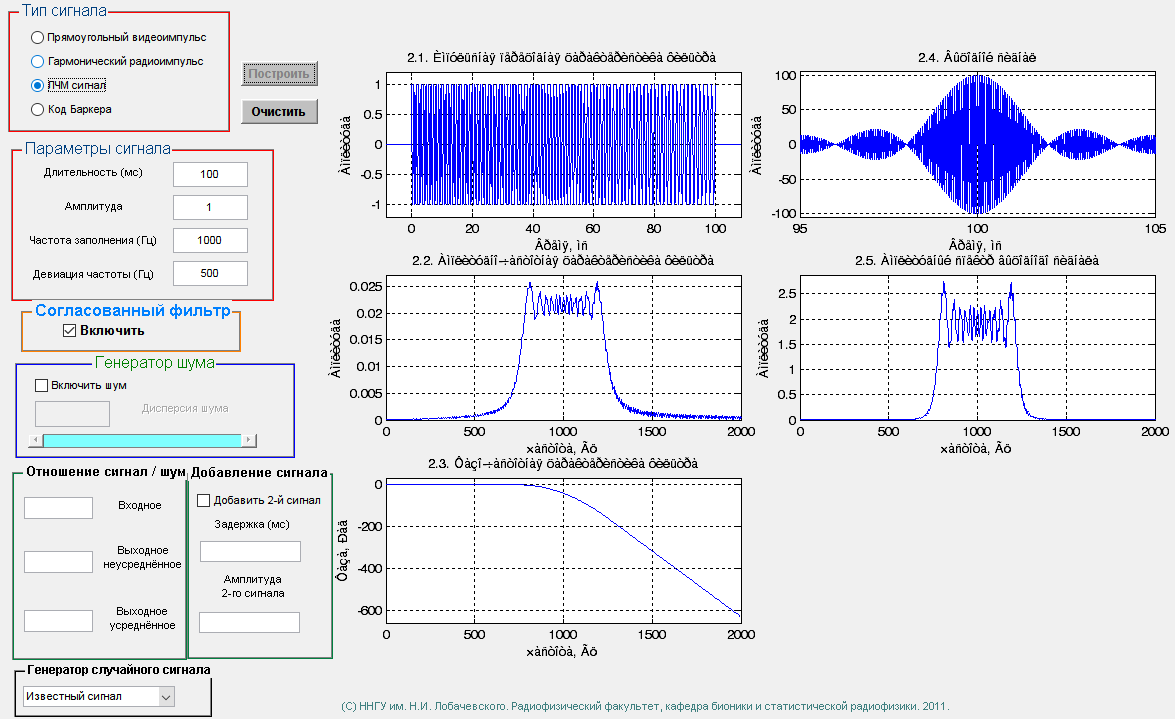
\includegraphics[width=0.9\linewidth]{imgs/task_2/t2s3_500.png}
    \caption{Девиация 500 Гц}
    \label{fig:task_2_3_500}
\end{figure}
\begin{figure}[H]
    \centering
    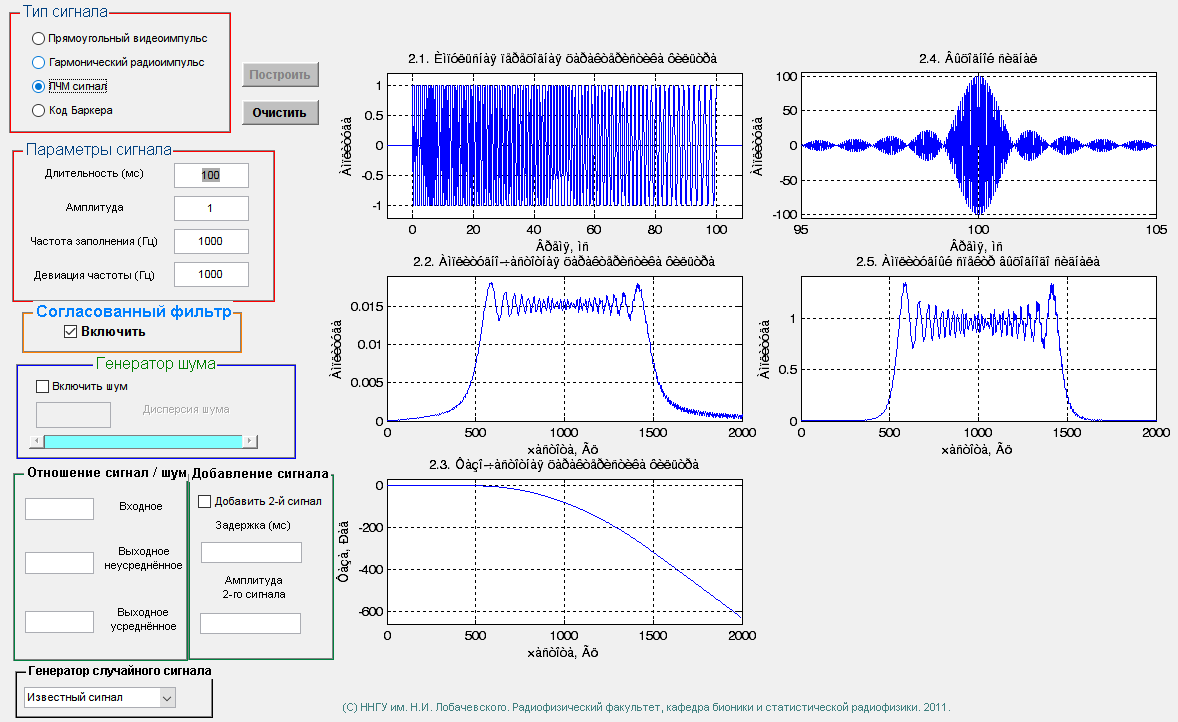
\includegraphics[width=0.9\linewidth]{imgs/task_2/t2s3_1000.png}
    \caption{Девиация 1000 Гц}
    \label{fig:task_2_3_1000}
\end{figure}

\begin{enumerate}
    \item 
    \item 
    \item 
    \item 
\end{enumerate}


\subsubsection{Код Баркера}
\begin{figure}[H]
    \centering
    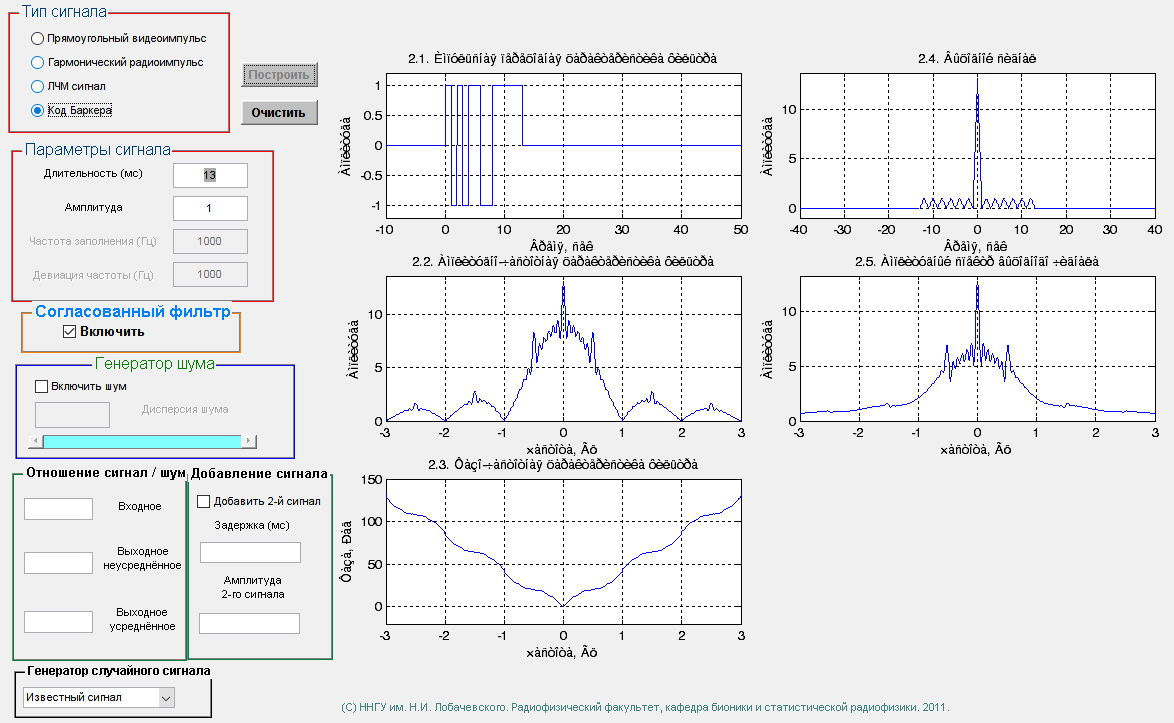
\includegraphics[width=0.9\linewidth]{imgs/task_2/t2s4_13.png}
    \caption{13 мс}
    \label{fig:task_2_4_13}
\end{figure}
\begin{figure}[H]
    \centering
    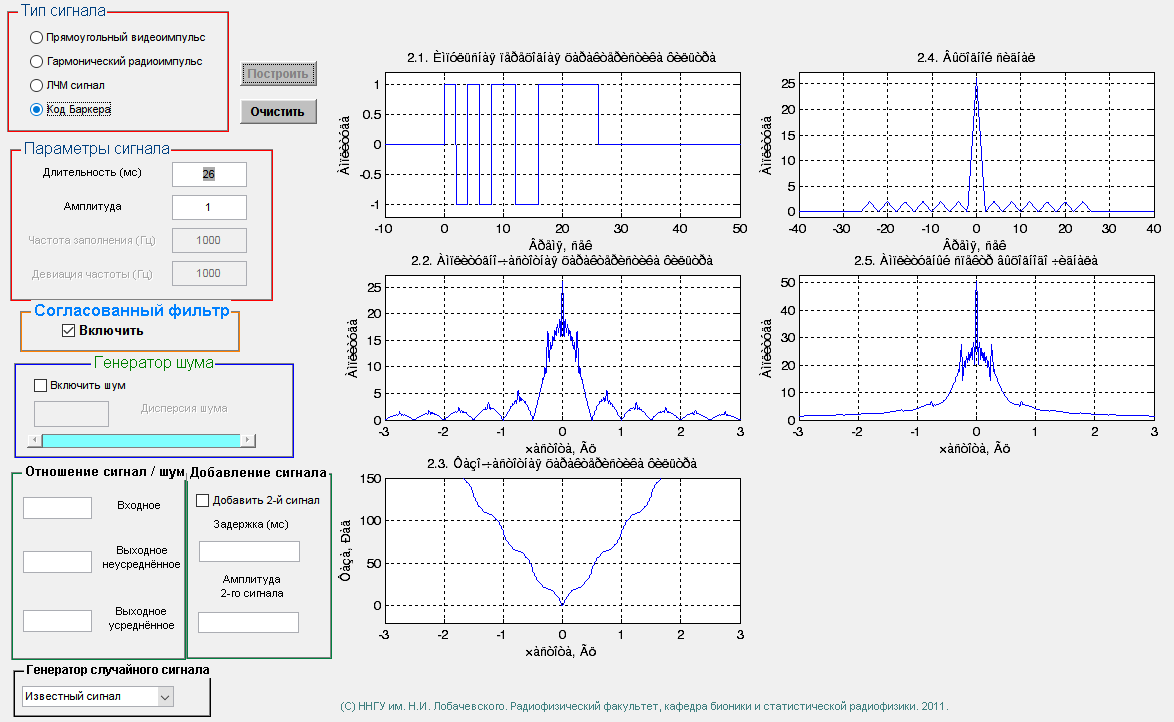
\includegraphics[width=0.9\linewidth]{imgs/task_2/t2s4_26.png}
    \caption{26 мс}
    \label{fig:task_2_4_26}
\end{figure}

\begin{enumerate}
    \item 
    \item 
    \item 
    \item 
\end{enumerate}